\documentclass[11pt, oneside]{article}   	% use "amsart" instead of "article" for AMSLaTeX format
\usepackage{geometry}                		% See geometry.pdf to learn the layout options. There are lots.
\geometry{letterpaper}                   		% ... or a4paper or a5paper or ... 
%\geometry{landscape}                		% Activate for rotated page geometry
%\usepackage[parfill]{parskip}    		% Activate to begin paragraphs with an empty line rather than an indent
\usepackage{graphicx}				% Use pdf, png, jpg, or eps§ with pdflatex; use eps in DVI mode
								% TeX will automatically convert eps --> pdf in pdflatex		
\usepackage{amssymb}

%SetFonts

%SetFonts

\graphicspath{ {./images/} } 			

\title{Population Pyramids}
\author{M: 941519}
%\date{}							% Activate to display a given date or no date

\begin{document}
\maketitle


\tableofcontents
\pagebreak
\section{Cos'è una "population pyramid"}
Una "population pyramid" è una illustrazione grafica che ci permette di visualizzare la distribuzione di una popolazione (che può essere un paese in particolare, una regione del mondo, o un continente). E' formata da due istogrammi che rappresentano le distribuzioni maschili e femminili di un paese, disposti simmetricamente intorno ad un'asse verticale che rappresenta le età.

La population pyramid è formata quindi da una serie di barre ad istogramma, la popolazione è rappresentata in proporzione o in valore assoluto dalla grandezza dell'asse orizzontale, ed le fasce di anni sono rappresentati dall'asse $y$.


\begin{center}
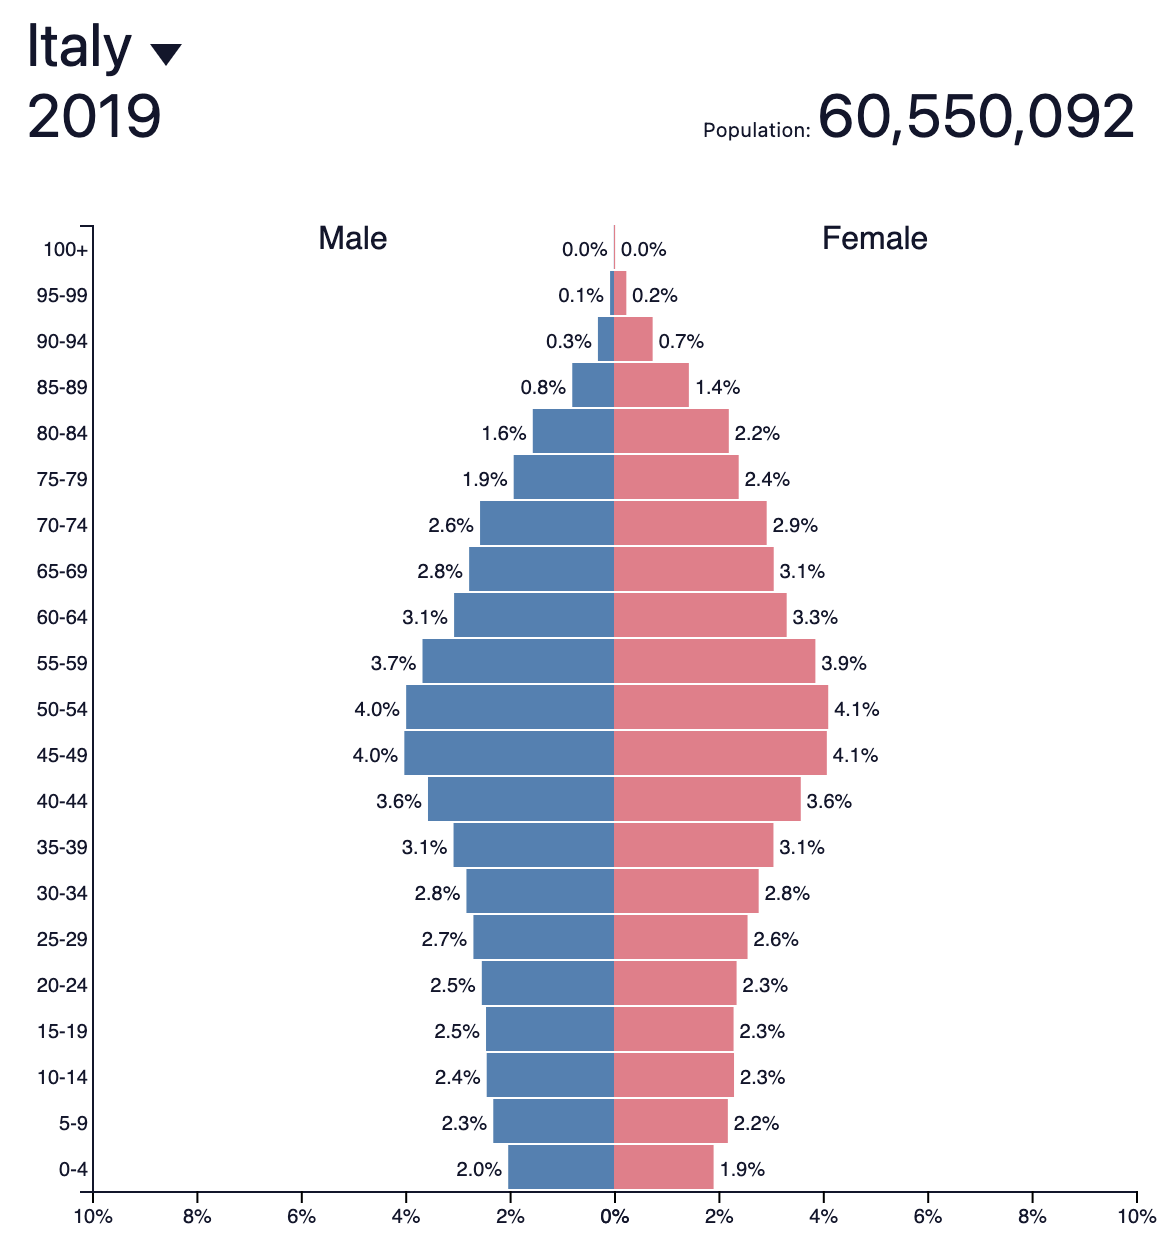
\includegraphics[scale=0.6]{pop}
\end{center}

\subsection{Perché è chiamata una "piramide"?}
L'origine del nome deriva dalla forma che questo grafico ha assunto per la maggior parte degli ultimi 200 anni, ovvero quella della piramide:
\begin{center}
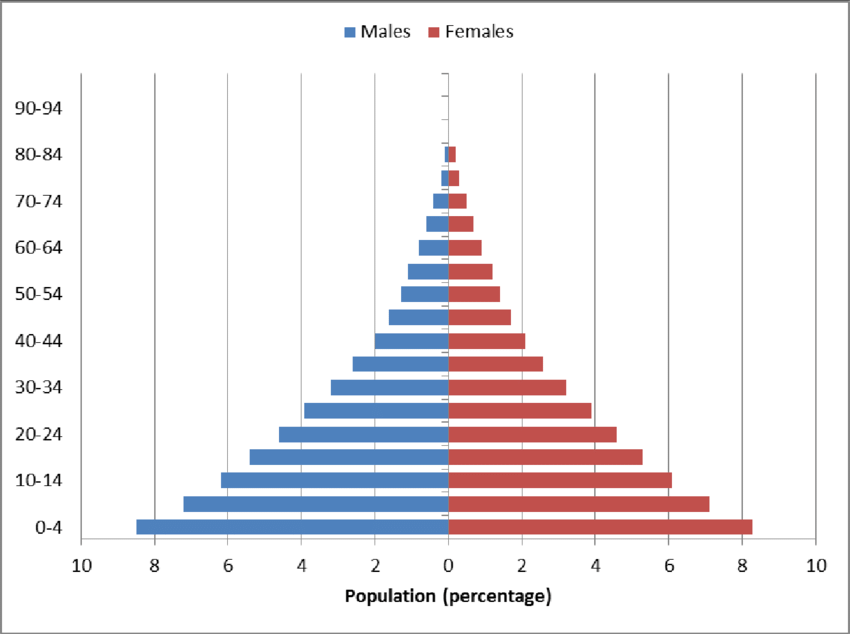
\includegraphics[scale=0.5]{pyramid.png}
\end{center}
Caratterizzata da una forma chiaramente piramidale, senza buoni contraccettivi e con una popolazione poco educata, la popolazione cresce man mano che ci spostiamo verso il basso del grafico, le famiglie sono quindi composte da molti bambini, che in gran parte non raggiunge neanche la maggiore età, e la popolazione diminuisce progressivamente per la mancanza di buona medicina e prevenzione. Quella comunque, è la "population pyramid" dell'Africa Subsahariana.


\section{I tipi di population pyramid}
\begin{itemize}
\item Constrictive o in compressione: rappresenta una piramide che ha meno persone nella fascia di persone giovani, ed è il tipo di forma assunta dalle parte delle società "sviluppate" , con un alto tasso di sviluppo, un tasso di mortalità infantile e natalità basso, con una popolazione in via di compressione.
\item Expansive o espansiva: rappresenta la piramide con forma piramidale, è caratterizzata da una fascia di persone giovani nettamente più grandi delle altre, e distingue paesi in cui i tassi di mortalità infantile e natalità sono alti, principalmente è la forma assunta dalle società in via di sviluppo.
\item Stationary o stazionaria: rappresenta una piramide pressoché bilanciata in tutte le fasce, questo va a caratterizzare società in cui i tassi di natalità sono bassi, ma pressoché costanti, con un alta qualità di vita.
\end{itemize}
\footnotesize{}
Qualcuno ha voglia di indovinare che tipo di piramide avranno i seguenti paesi:?
Burkina Faso (espansiva), Stati Uniti (stazionaria), Italia (in compressione), Norvegia (stazionaria)

\normalsize{}

\begin{center}
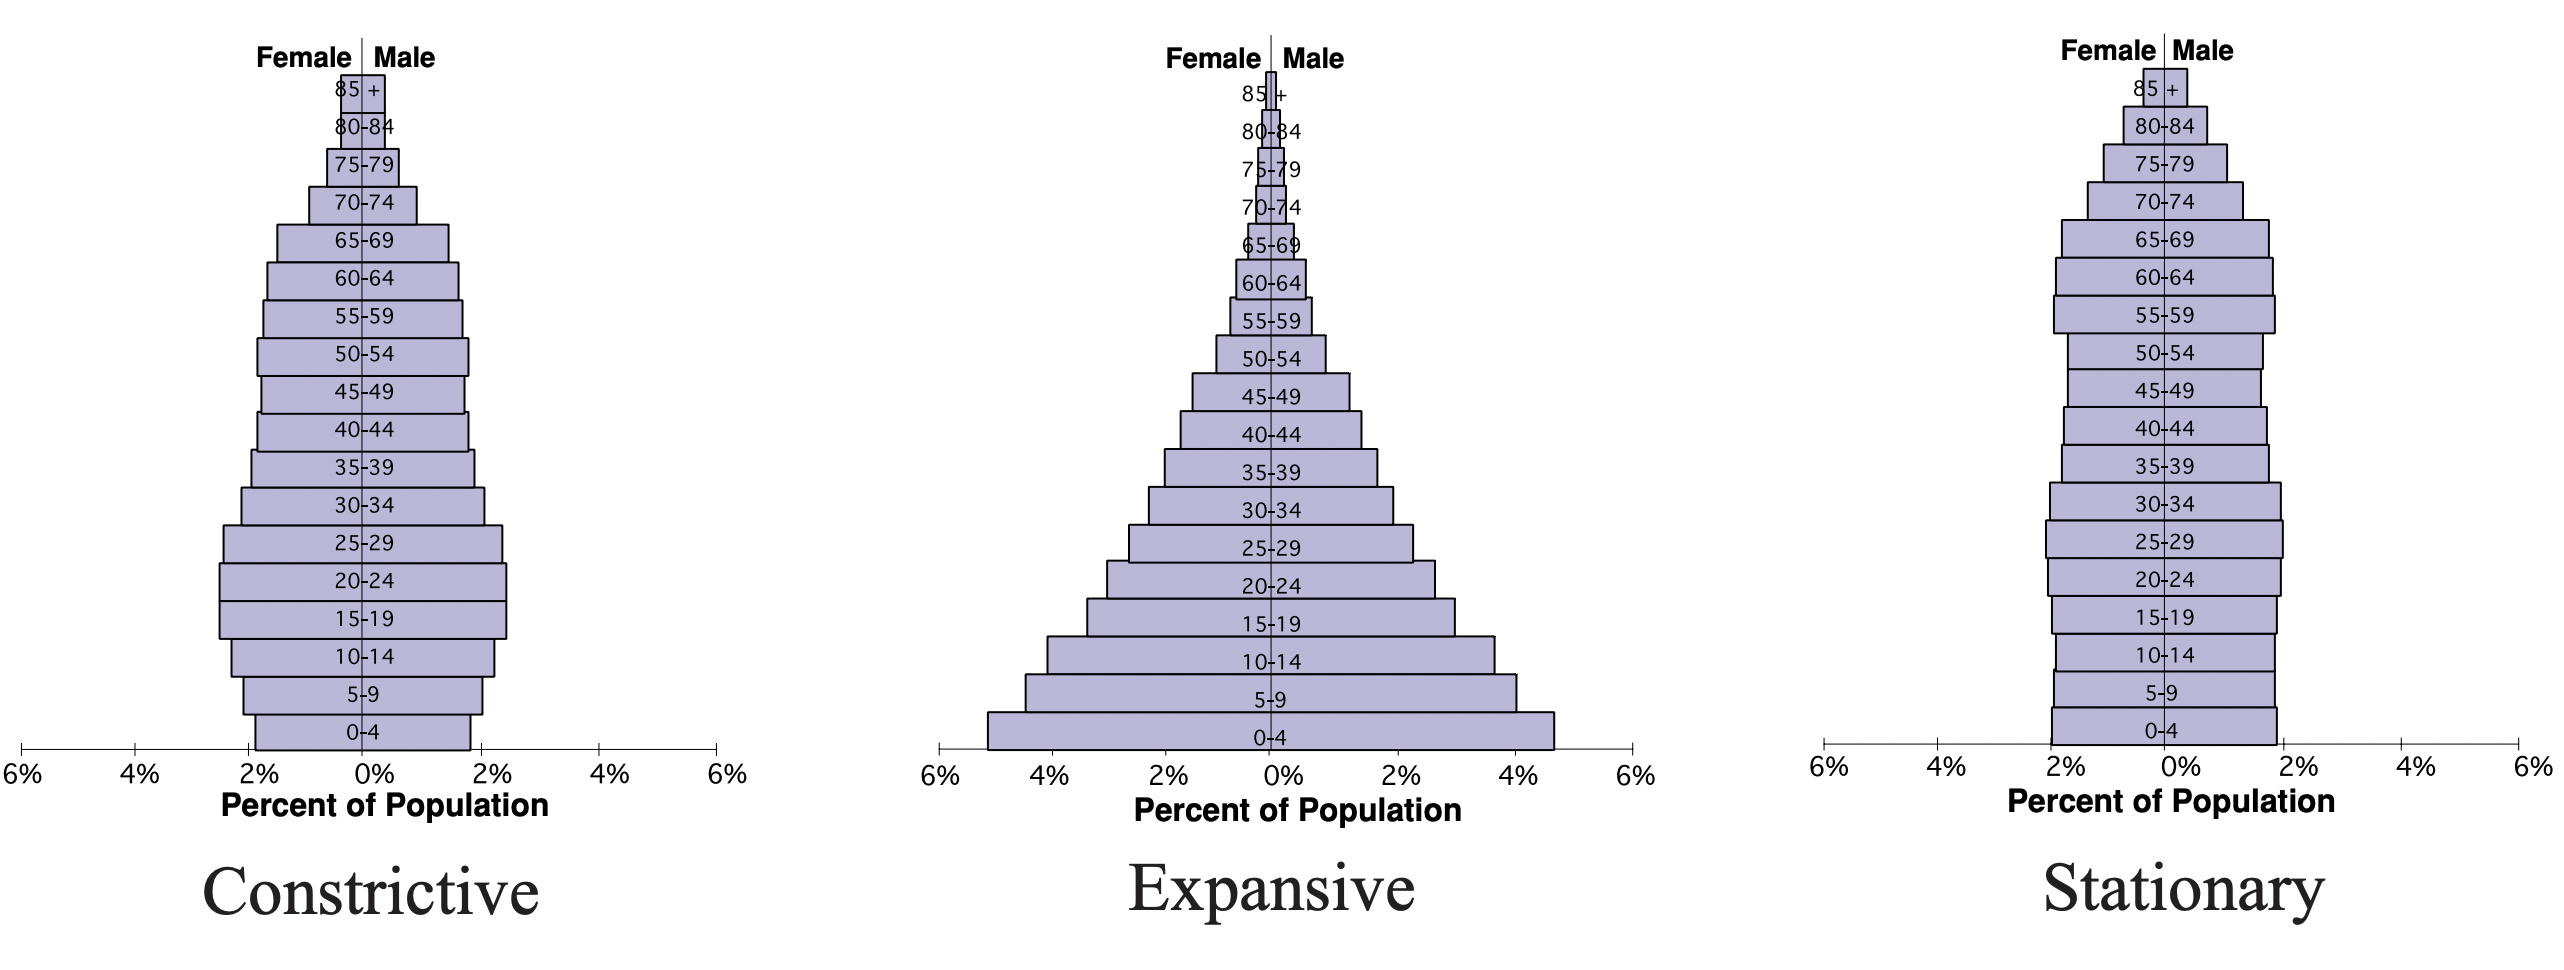
\includegraphics[scale=0.3]{types}
\end{center}

\section{I dati necessari per costruire una "population pyramid"}
Per costruire una population pyramid abbiamo bisogno prima di tutto della popolazione totale in uno specifico anno, nel nostro esempio abbiamo preso l'Italia nell'anno 2019, e la popolazione totale è di $60.550.092$. \\
Il secondo dato fondamentale che ci serve è la proporzione, rispetto alla popolazione totale, della popolazione per ogni "age bracket". Questo dato va a rispondere alla domanda: \emph{"quante persone, maschio e femmina, vi erano, in percentuale, rispetto alla popolazione totale ?"}. Questo dato ci permette di dimensionare le varie barre del nostro grafico\\
L'ultimo dato fondamentale è la proporzione tra maschi e femmine, rispetto ad ogni "age bracket", che ci permette dimensionare, in proporzione, i maschi e le femmine.



\section{Esempio di costruzione utilizzando python}

\subsection{Costruzione di diagramma a barre}
Siccome il dataset raccoglie già i valori di popolazione per age bracket, il primo grafico che possiamo andare a costruire è il bar chart. Il bar chart è un grafico formato da rettangoli la cui altezza è dimensionata in base a valore che vanno a rappresentare. 

Siccome vogliamo lavorare con un subset dei dati presenti, effettuiamo uno slicing sul dataframe iniziale, e chiamiamo la funzione plot, con argument \emph{kind = 'bar'} per costruire il diagramma a barre.
\begin{center}
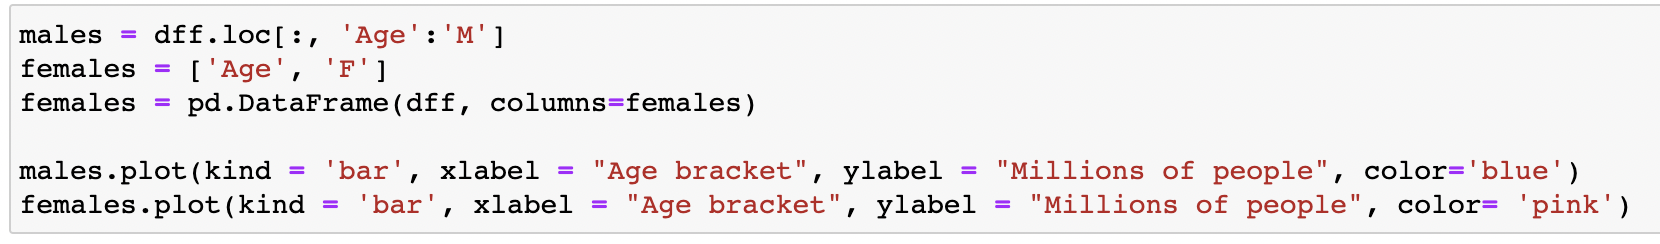
\includegraphics[scale=0.6]{bar}
\end{center}
Coloriamo i grafici di blue e rosso rispettivamente in base al sesso:
\begin{center}
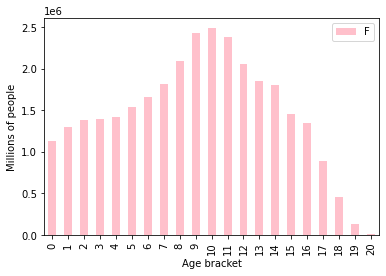
\includegraphics[scale=0.6]{females}
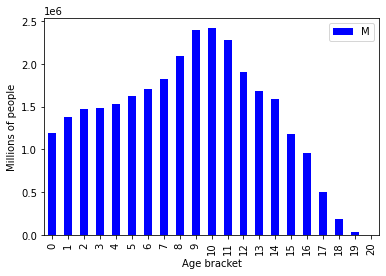
\includegraphics[scale=0.6]{males}
\end{center}

\subsubsection{Costruzione della population pyramid}
Utilizziamo un dataset fornito da \emph{https://www.populationpyramid.net/}:
\begin{center}
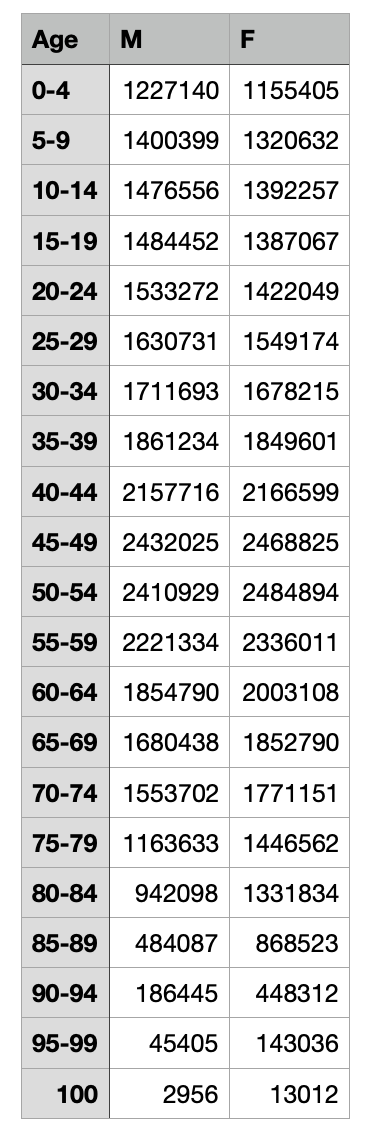
\includegraphics[scale=0.6]{popitaly}
\end{center}
Andiamo ad importare il dataset all'interno del notebook:
\begin{center}
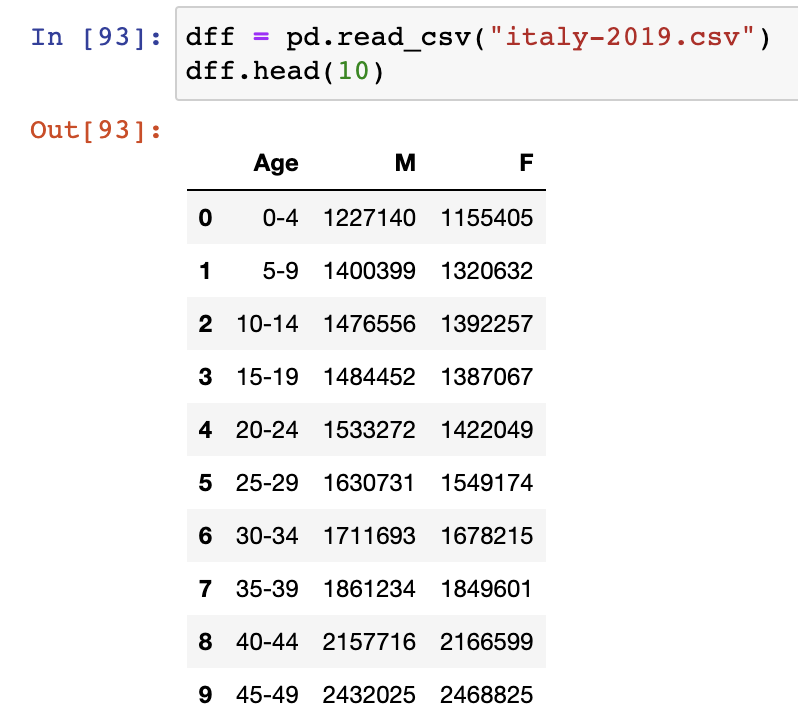
\includegraphics[scale=0.6]{popitaly2}
\end{center}
Costruiamo due liste, una per i maschi ed una per le femmine, raccogliendo i valori in base all'age bracket:
\begin{center}
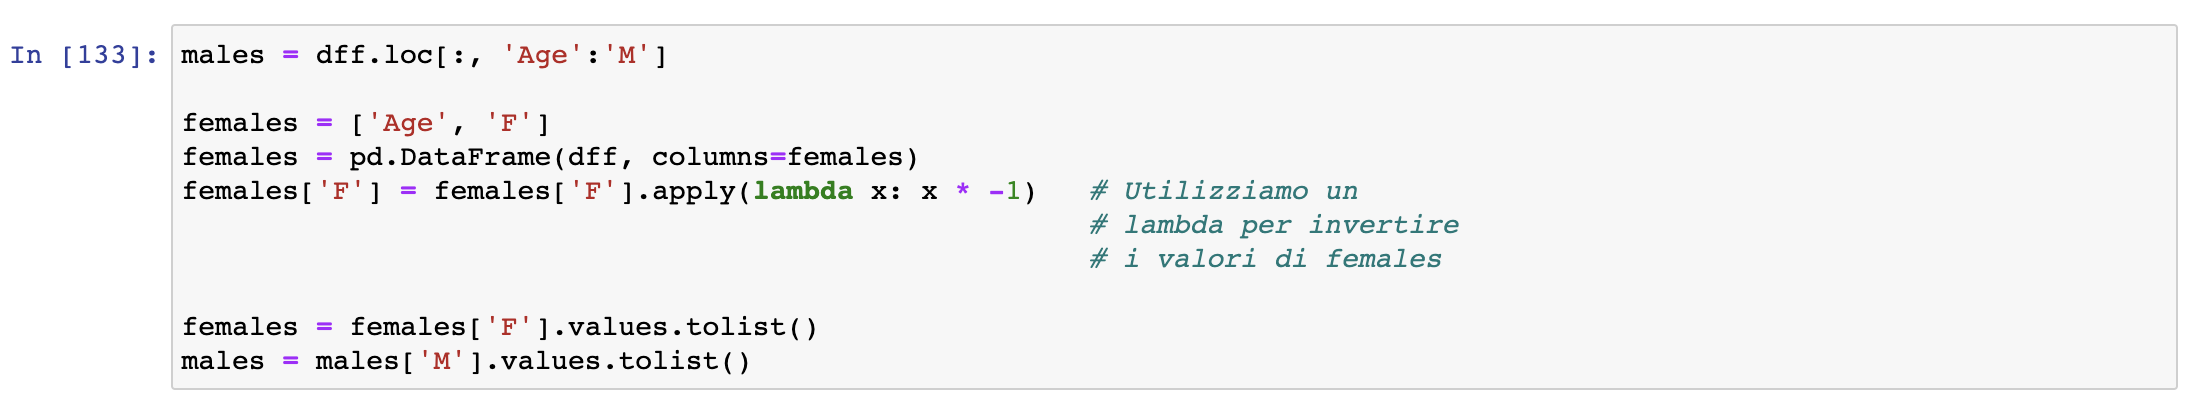
\includegraphics[scale=0.4]{popitaly3}
\end{center}
Creiamo un dataframe con headers: "Age", "Males", "Females", e utilizziamo le liste precedentemente create come input. utilizziamo quindi la libreria seaborn (basata su matplotlib) per creare la nostra population pyramid:
\begin{center}
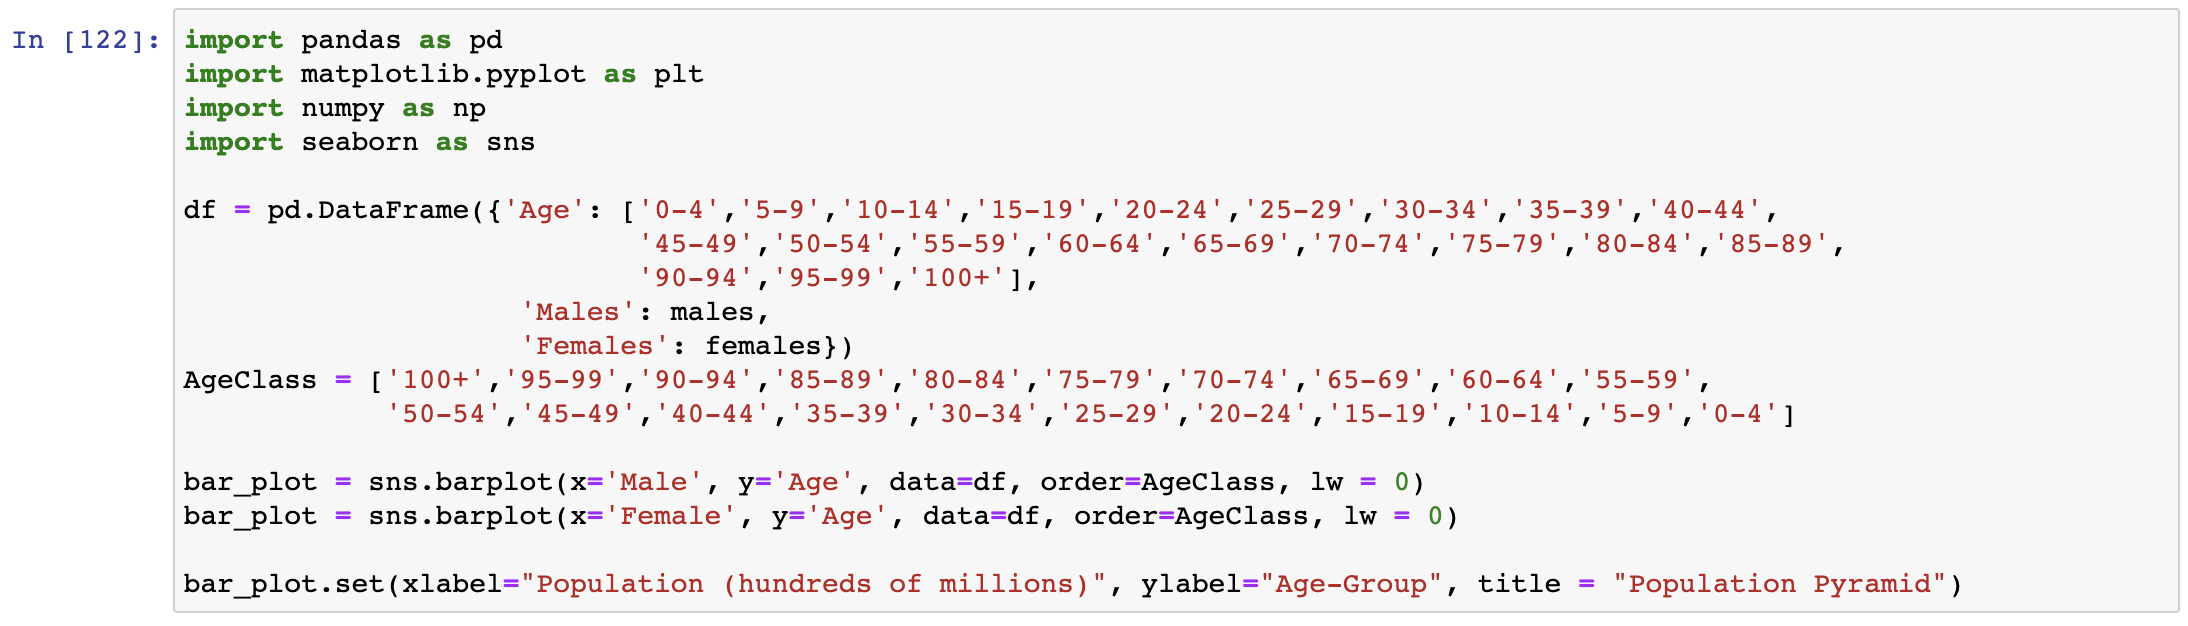
\includegraphics[scale=0.4]{popitaly4}
\end{center}
Il risultato finale è il seguente:
\begin{center}
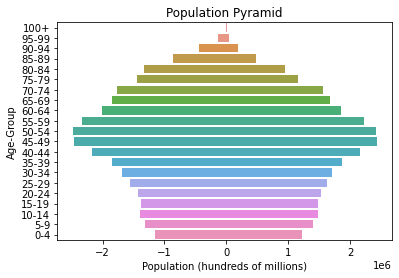
\includegraphics[scale=1]{popitaly5}
\end{center}
\subsection{Dependancy ratio}
Il dependancy ratio è un indicatore che va a definire il rapporto tra la popolazione "dipendente" e quella "non dipendente". Per popolazione dipendente si intende la popolazione con età compresa tra 0 e 14, e da 65+.
Questa suddivisione è fatta per misurare la pressione sulla popolazione produttiva, e quella non produttiva. Un dependancy ratio più basso -di norma- si materializza in pensioni più alte, ed un sistema economico più salutare di uno con un dependancy ratio più alto, che solitamente si traduce in un maggiore stress sulla popolazione lavoratrice.

Dependancy ratio o indice di dipendenza è un indicatore demografico che va a rappresentare il rapporto tra le persone non più presenti nella manodopera di un paese, e quelli nella manodopera. E' quindi un indicatore che va a rappresentare la pressione sulla popolazione produttiva, higher is worse. Un basso tasso di dipendenza -solitamente- significa che ci sono meno persone da supportare, e quindi migliori pensioni, migliore sanità, più reinvestimenti nella società.


L'equazione della dependancy ratio è cosi definita:
\begin{center}
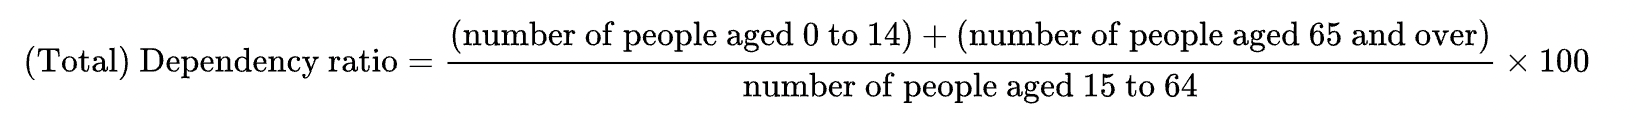
\includegraphics[scale=0.5]{dependancy}
\end{center}
Andiamo a costruire un grafico dell'andamento del dependancy ratio dell'Italia dal 2000 al 2020:
Andiamo a ciclare sui vari dataset, facendo un slicing per mettere in risalto i valori maschili e femmine di porzioni attive ed inattive. Utilizziamo poi la formula per calcolare il dependancy ratio dell'anno e lo inseriamo nella lista
\begin{center}
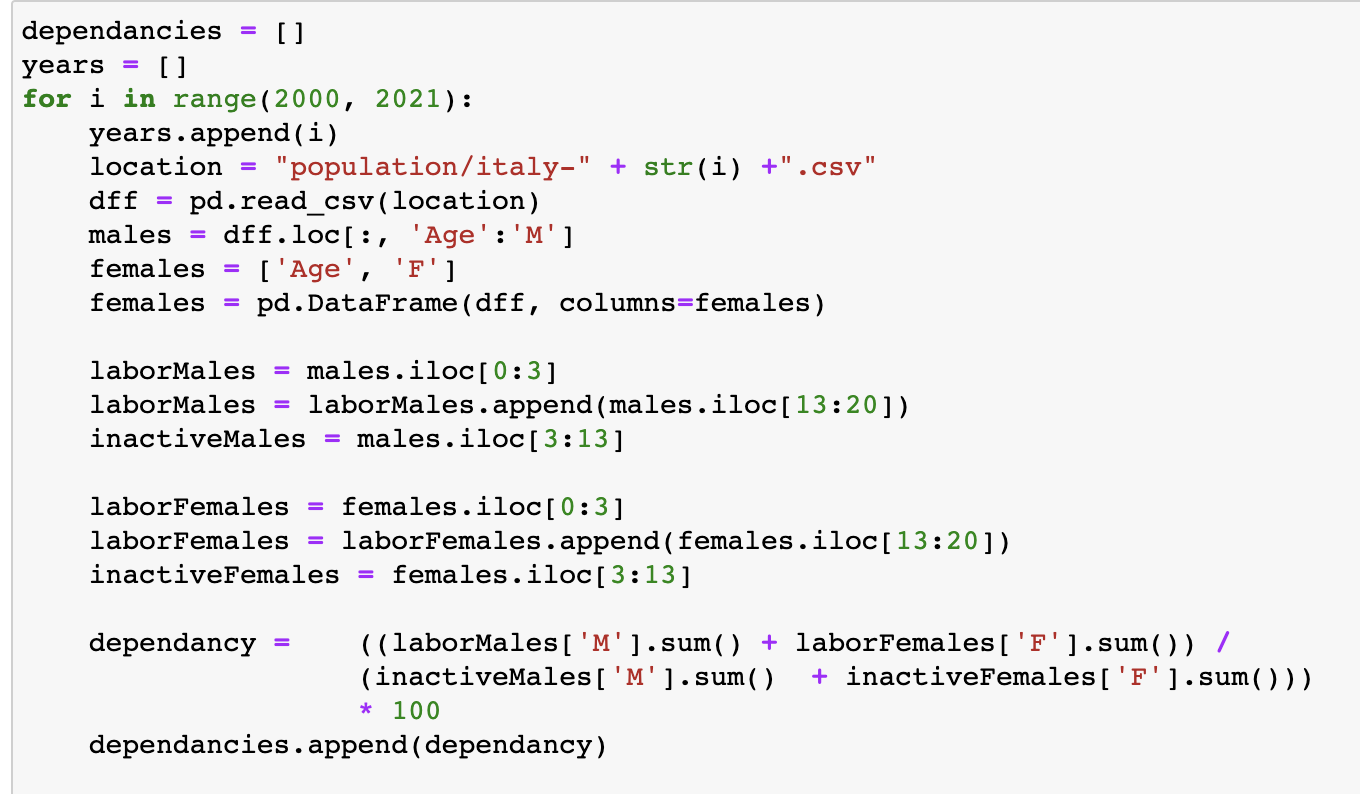
\includegraphics[scale=0.5]{dep1}
\end{center}
Prepariamo il line chart mettendo dei pallini per mettere in risalto i valori per anno.
\begin{center}
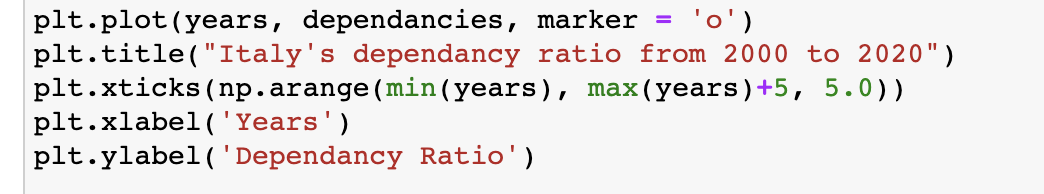
\includegraphics[scale=0.5]{dep2}
\end{center}
Ed ecco il grafico finale:
\begin{center}
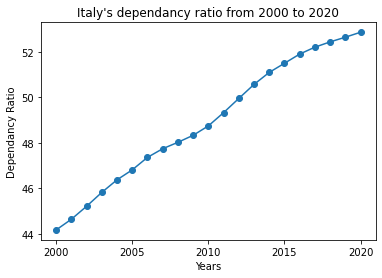
\includegraphics[scale=0.8]{dep3}
\end{center}

\section{Cosa ci dice una "population pyramid"}
\subsection{Un'appendice sull'età}
\emph{Qual'è il miglior indicatore per prevedere il comportamento di una "persona media" ed il suo contributo alla società?}\\
Ci sono molte risposte a questa domanda, il background culturale, la professione, le condizioni sociali, la propensione al risparmio di una società. L'europeo medio ad esempio risparmia di più rispetto ad un americano medio, il finanziere che guadagna 100.000\$ l'anno investe di più (anche solo perché ha più disposable income) di un meccanico che raggiunge a malapena il fine mese, e così via.\\
C'è tuttavia un dato che ci permette di prevedere, in maniera pressoché accurata, il contributo di una persona al proprio paese: l'età.

\subsubsection{Perché l'età è un indicatore così importante}
Utilizziamo la nostra "population pyramid", e consideriamo la bracket di popolazione con età superiore a 65 anni circa. Questa categoria è rappresentata solitamente dai pensionati, che hanno terminato la propria carriera lavorativa, spendono poco, investono in maniera prudente e non contribuiscono più alle casse dello stato. \\

Il secondo gruppo che ci interessa è la bracket di popolazione con età compresa tra i 30 e i 65 anni. Questo bracket di popolazione rappresenta il "motore" di un paese, rappresenta il lavoratore medio che percepisce uno stipendio, spende, risparmia, e contribuisce alle casse dello stato. Durante questi anni la persona media raggiunge il massimo potenziale economico, facendo carriera, comprando case, macchine, e mettendo su famiglia. E' questo quindi il motivo per cui possiamo considerare questo bracket di popolazione come la risorsa più importante di un paese, più importante anche delle risorse naturali, e della posizione geografica.\\

Il terzo gruppo che ci interessa è la bracket di popolazione con età compresa tra i 15 ed i 30 anni. Questo bracket di popolazione è principalmente composta da persone che stanno per terminare la propria carriera formativa, e che stanno per entrare nel mondo del lavoro.
Durante questi anni la persona media non guadagna molto, vive solitamente con i genitori, e ha bisogno di prestiti per finanziare rette universitarie, o per comprare la prima casa.\\

L'ultimo gruppo che ci interessa è la bracket di popolazione con età inferiore ai 15 anni. Questo bracket di popolazione è la "più inutile" per un paese, formata da studenti e bambini che non contribuiscono ad una economicamente ad una società, ed invece costano molto alle famiglie sotto forma di mantenimento, pannolini etc.\\

Chiaramente la caratterizzazione che abbiamo non può essere applicato ad una qualsiasi società nel mondo e dipende strettamente dal livello di sviluppo di un paese, dalla geografia, dal livello di sviluppo della sanità, economia, e da una miriade di altri fattori. 

\section{Estensione delle population pyramids}
\begin{itemize}
\item Population pyramid colorate maschio e femmina\\
L'abbiamo vista in precedenza, ed è la più semplice delle varianti, sono population pyramids in cui le barre sono colorate a seconda del sesso della popolazione.
\item Population pyramid con surplus
Sono un'estensione della precedente, in cui oltre al colorare il sesso delle barre, coloriamo in maniera differente il surplus delle barre rispetto all'altro sesso, in questo modo possiamo visualizzare in maniera semplice la quantità di maschi, o femmine, in più in un paese.
\begin{center}
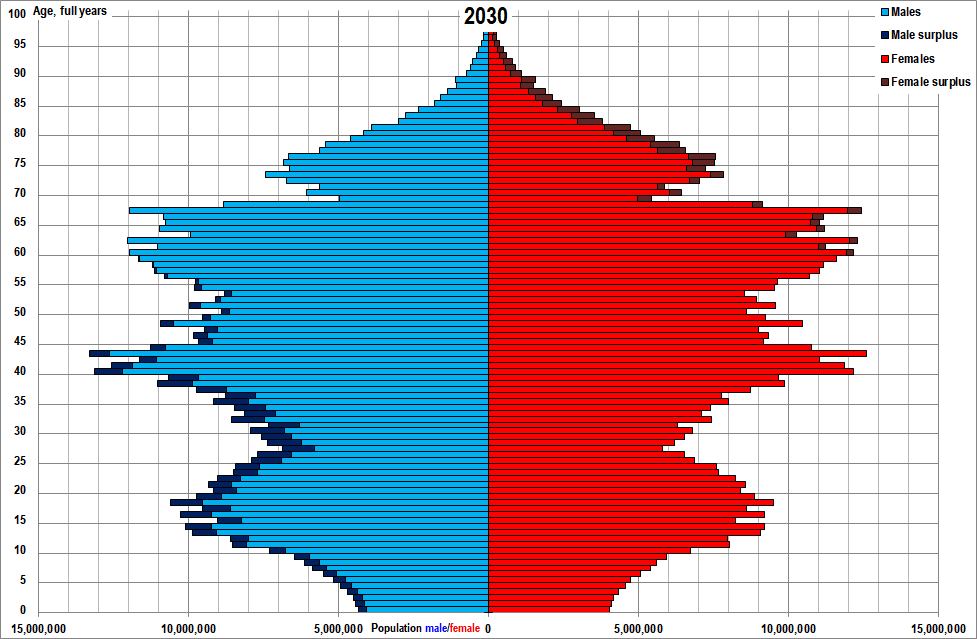
\includegraphics[scale=0.6]{china}
\end{center}
\item Animazioni con population pyramids\\
Andiamo a costruire un'animazione con il dataset che abbiamo.
Siccome il nostro dataset va dal 2000 al 2020, estendiamo il programmino creato in precedenza aggiungendo un ciclo range, e salviamo con nome ogni grafico prodotto, dal 2000 al 2020.

\begin{center}
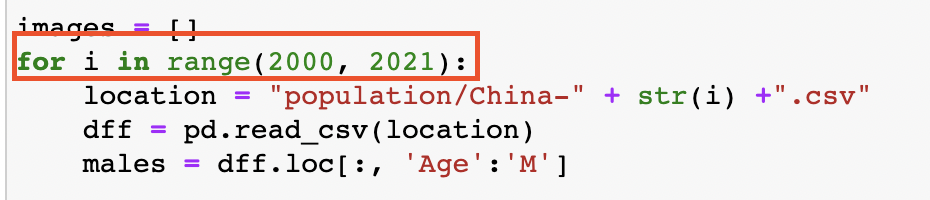
\includegraphics[scale=0.5]{china1}


\includegraphics[scale=0.55]{china2}

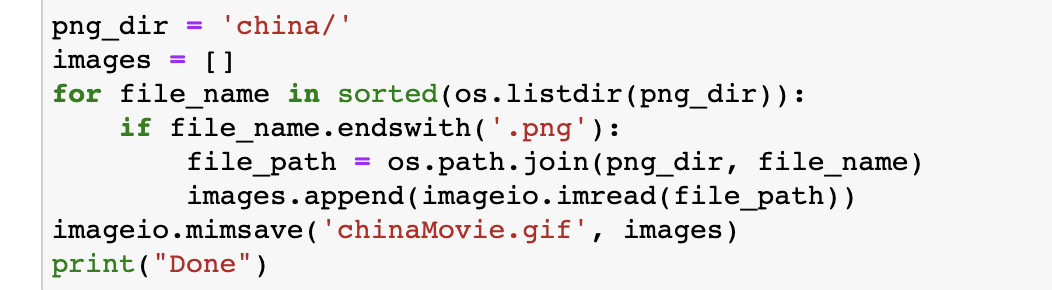
\includegraphics[scale=0.5]{china3}
\end{center}
Con le immagini generate utilizziamo un piccolo script basato su \emph{imageio} per generare una .gif.\\
Questo tipo di animazione ci permette di vedere in maniera dinamica lungo gli anni l'andamento della popolazione, in particolare possiamo vedere come la popolazione -nei paesi in via di sviluppo-, si sposta tendenzialmente verso l'alto allontanandosi sempre più da una piramide, ed avvicinandosi ad una campana; mentre nei paesi il cui l'indice di sviluppo è basso il grafico rimane una piramide, indicatore di come lo sviluppo non stia tenendo passo.

\item Predizioni sul futuro con population pyramids\\
Un qualcosa che ci stanno pregando di fare le animazioni precedenti è quello di estenderle, per darci una visione del futuro. In base all'andamento demografico di un paese è quindi possibile estendere il grafico lungo gli anni.

\end{itemize}













\end{document}  